\section{Программный пакет \texttt{nudisxs}}

\subsection{Происхождение и назначение}

Пакет \texttt{nudisxs}~\cite{nudisxs2022} представляет собой программный инструмент на языке Python, предназначенный для вычисления сечений нейтрино-нуклонного взаимодействия в области глубоконеупругого рассеяния согласно формуле~\eqref{eq:xsec_general}. Ядро вычислений основано на пакете \texttt{XsDis}, написанном на языке Fortran В.~А.~Наумовым и К.~С.~Кузьминым (см., например,~\cite{nudisxs2022}). Первоначально \texttt{XsDis} рассчитывал DIS-сечения для фиксированных партонных функций, и впоследствии был преобразован нами в современный Python-модуль \texttt{nudisxs}, поддерживающий динамическую загрузку партонных распределений из библиотеки \texttt{LHAPDF6}~\cite{aartsenLHAPDF2020}.

Пакет \texttt{nudisxs} позволяет рассчитывать дважды дифференциальные сечения по переменным Бьёркена $x$ и $y$, дифференциальные сечения по одной переменной и полные сечения взаимодействия для широкого диапазона энергий — от нескольких сотен МэВ до $10^{15}$~ГэВ. Пакет предназначен для использования в задачах нейтринной астрофизики и моделирования событий в нейтринных телескопах. Пакет находится в открытом доступе и может быть легко интегрирован в любые исследовательские проекты.


Пакет реализован на языке Python 3, активно использует библиотеки \texttt{NumPy}~\cite{2020NumPy-Array} и \texttt{SciPy}~\cite{2020SciPy-NMeth}, а также библиотеку \texttt{vegas}~\cite{lepageVegas2021} для многомерного Монте-Карло интегрирования. Благодаря этому он обладает высокой производительностью и удобен в использовании для анализа, тестирования и встраивания в более крупные симуляционные цепочки.

Пакет \texttt{nudisxs} является самостоятельным компонентом генератора нейтринных событий \texttt{NuPropagator}, который, в свою очередь, интегрируется в более общий фреймворк \href{https://pypi.org/project/ntsim/}{\texttt{NTSim}}, который разрабатывается эксперимента Baikal-GVD и других нейтринных телескопов.

\subsection{Структура и функциональность}

Логическая архитектура пакета \texttt{nudisxs} представлена на рис.~\ref{fig:nudisxs1}. Основные компоненты и зависимости включают:

\begin{enumerate}
    \item Загрузка партонных функций из библиотеки \texttt{LHAPDF6}, которые используются для построения структурных функций $F_i(x, Q^2)$, необходимых для расчёта сечений.
    
    \item Модуль \texttt{dis} реализует интерфейс пользователя: здесь задаются тип лептона (нейтрино/антинейтрино), мишень (протон, нейтрон или изоскаляр), энергия нейтрино, минимальное значение $Q^2$, используемые партонные распределения и другие параметры модели.
    
    \item Модули \texttt{xs\_cc} и \texttt{xs\_nc} возвращают дважды дифференциальные сечения для заряженного и нейтрального токов, соответственно. 
    
    \item Часть исходного кода, написанного на Fortran, остаётся доступной через интерфейс \texttt{f2py} и обеспечивает быстрые и проверенные временем вычисления основных выражений для сечений.
    
    \item Интерполяция PDF и структурных функций, а также численные процедуры, реализованы с помощью \texttt{SciPy}.
\end{enumerate}

\begin{figure}[!h]
\centering
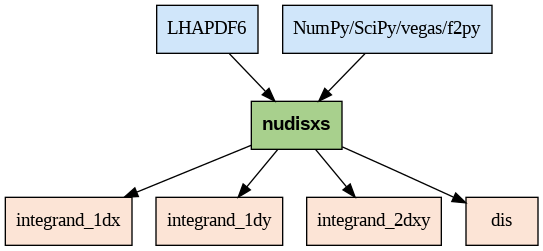
\includegraphics[width=\linewidth]{images/nudisxs_diagram.png}
\caption{Структура программного пакета \texttt{nudisxs} и его зависимости.}
\label{fig:nudisxs1}
\end{figure}

Пакет занимает менее 120~КБ и поставляется через платформу \texttt{PyPI} как открытое программное обеспечение. Его легко установить и интегрировать в любые пользовательские симуляционные цепочки. В рамках настоящей работы пакет \texttt{nudisxs} использован для построения всех сечений, представленных на рис.~\ref{fig:xsec_2d}–\ref{fig:xsec_total}.


%NTSim - один из таких пакетов моделирования, создаваемый для эксперимента Baikal-GVD. Он представляет собой комплекс инструментов, написанных на Python, который позволяет не только моделировать нейтринные события, но и выполнять расчеты для атмосферных мюонов, а также анализировать данные о взаимодействии частиц с детекторами. Программа включает цепочку моделирования, которая охватывает все этапы: от генерации первичных взаимодействий до анализа данных. В отличие от специализированных пакетов, ориентированных на конкретные типы телескопов, NTSim поддерживает моделирование различных конфигураций детекторов, что делает его универсальным инструментом. NTSim позволяет учитывать широкий спектр физических процессов, включая взаимодействие нейтрино с веществом, распространение черенковского излучения и влияние среды (например, воды или льда) . Это повышает точность моделирования по сравнению с более простыми методами. Благодаря оптимизации алгоритмов и использованию современных численных методов, NTSim обеспечивает высокую скорость расчетов даже при моделировании больших объемов данных. 
%NTSim значительно улучшает точность моделирования за счет нескольких ключевых факторов:
 %\begin{enumerate}
 %    \item Программный пакет использует современные модели для описания взаимодействия нейтрино с веществом, что позволяет минимизировать ошибки при расчете энергий и направлений частиц.
%     \item NTSim включает модули для моделирования фоновых шумов, таких как биолюминесценция в воде или радиационные эффекты в льду. Это помогает более точно выделять сигналы от нейтрино.
%     \item Также данный пакет использует специальные методы распространения фотонов,  разработанные специально для NTSim и сильно ускоряющих всю цепочку моделирования. 
% \end{enumerate}  
